% Options for packages loaded elsewhere
\PassOptionsToPackage{unicode}{hyperref}
\PassOptionsToPackage{hyphens}{url}
%
\documentclass[
]{article}
\usepackage{amsmath,amssymb}
\usepackage{lmodern}
\usepackage{iftex}
\ifPDFTeX
  \usepackage[T1]{fontenc}
  \usepackage[utf8]{inputenc}
  \usepackage{textcomp} % provide euro and other symbols
\else % if luatex or xetex
  \usepackage{unicode-math}
  \defaultfontfeatures{Scale=MatchLowercase}
  \defaultfontfeatures[\rmfamily]{Ligatures=TeX,Scale=1}
\fi
% Use upquote if available, for straight quotes in verbatim environments
\IfFileExists{upquote.sty}{\usepackage{upquote}}{}
\IfFileExists{microtype.sty}{% use microtype if available
  \usepackage[]{microtype}
  \UseMicrotypeSet[protrusion]{basicmath} % disable protrusion for tt fonts
}{}
\makeatletter
\@ifundefined{KOMAClassName}{% if non-KOMA class
  \IfFileExists{parskip.sty}{%
    \usepackage{parskip}
  }{% else
    \setlength{\parindent}{0pt}
    \setlength{\parskip}{6pt plus 2pt minus 1pt}}
}{% if KOMA class
  \KOMAoptions{parskip=half}}
\makeatother
\usepackage{xcolor}
\usepackage[margin=1in]{geometry}
\usepackage{color}
\usepackage{fancyvrb}
\newcommand{\VerbBar}{|}
\newcommand{\VERB}{\Verb[commandchars=\\\{\}]}
\DefineVerbatimEnvironment{Highlighting}{Verbatim}{commandchars=\\\{\}}
% Add ',fontsize=\small' for more characters per line
\usepackage{framed}
\definecolor{shadecolor}{RGB}{248,248,248}
\newenvironment{Shaded}{\begin{snugshade}}{\end{snugshade}}
\newcommand{\AlertTok}[1]{\textcolor[rgb]{0.94,0.16,0.16}{#1}}
\newcommand{\AnnotationTok}[1]{\textcolor[rgb]{0.56,0.35,0.01}{\textbf{\textit{#1}}}}
\newcommand{\AttributeTok}[1]{\textcolor[rgb]{0.77,0.63,0.00}{#1}}
\newcommand{\BaseNTok}[1]{\textcolor[rgb]{0.00,0.00,0.81}{#1}}
\newcommand{\BuiltInTok}[1]{#1}
\newcommand{\CharTok}[1]{\textcolor[rgb]{0.31,0.60,0.02}{#1}}
\newcommand{\CommentTok}[1]{\textcolor[rgb]{0.56,0.35,0.01}{\textit{#1}}}
\newcommand{\CommentVarTok}[1]{\textcolor[rgb]{0.56,0.35,0.01}{\textbf{\textit{#1}}}}
\newcommand{\ConstantTok}[1]{\textcolor[rgb]{0.00,0.00,0.00}{#1}}
\newcommand{\ControlFlowTok}[1]{\textcolor[rgb]{0.13,0.29,0.53}{\textbf{#1}}}
\newcommand{\DataTypeTok}[1]{\textcolor[rgb]{0.13,0.29,0.53}{#1}}
\newcommand{\DecValTok}[1]{\textcolor[rgb]{0.00,0.00,0.81}{#1}}
\newcommand{\DocumentationTok}[1]{\textcolor[rgb]{0.56,0.35,0.01}{\textbf{\textit{#1}}}}
\newcommand{\ErrorTok}[1]{\textcolor[rgb]{0.64,0.00,0.00}{\textbf{#1}}}
\newcommand{\ExtensionTok}[1]{#1}
\newcommand{\FloatTok}[1]{\textcolor[rgb]{0.00,0.00,0.81}{#1}}
\newcommand{\FunctionTok}[1]{\textcolor[rgb]{0.00,0.00,0.00}{#1}}
\newcommand{\ImportTok}[1]{#1}
\newcommand{\InformationTok}[1]{\textcolor[rgb]{0.56,0.35,0.01}{\textbf{\textit{#1}}}}
\newcommand{\KeywordTok}[1]{\textcolor[rgb]{0.13,0.29,0.53}{\textbf{#1}}}
\newcommand{\NormalTok}[1]{#1}
\newcommand{\OperatorTok}[1]{\textcolor[rgb]{0.81,0.36,0.00}{\textbf{#1}}}
\newcommand{\OtherTok}[1]{\textcolor[rgb]{0.56,0.35,0.01}{#1}}
\newcommand{\PreprocessorTok}[1]{\textcolor[rgb]{0.56,0.35,0.01}{\textit{#1}}}
\newcommand{\RegionMarkerTok}[1]{#1}
\newcommand{\SpecialCharTok}[1]{\textcolor[rgb]{0.00,0.00,0.00}{#1}}
\newcommand{\SpecialStringTok}[1]{\textcolor[rgb]{0.31,0.60,0.02}{#1}}
\newcommand{\StringTok}[1]{\textcolor[rgb]{0.31,0.60,0.02}{#1}}
\newcommand{\VariableTok}[1]{\textcolor[rgb]{0.00,0.00,0.00}{#1}}
\newcommand{\VerbatimStringTok}[1]{\textcolor[rgb]{0.31,0.60,0.02}{#1}}
\newcommand{\WarningTok}[1]{\textcolor[rgb]{0.56,0.35,0.01}{\textbf{\textit{#1}}}}
\usepackage{graphicx}
\makeatletter
\def\maxwidth{\ifdim\Gin@nat@width>\linewidth\linewidth\else\Gin@nat@width\fi}
\def\maxheight{\ifdim\Gin@nat@height>\textheight\textheight\else\Gin@nat@height\fi}
\makeatother
% Scale images if necessary, so that they will not overflow the page
% margins by default, and it is still possible to overwrite the defaults
% using explicit options in \includegraphics[width, height, ...]{}
\setkeys{Gin}{width=\maxwidth,height=\maxheight,keepaspectratio}
% Set default figure placement to htbp
\makeatletter
\def\fps@figure{htbp}
\makeatother
\setlength{\emergencystretch}{3em} % prevent overfull lines
\providecommand{\tightlist}{%
  \setlength{\itemsep}{0pt}\setlength{\parskip}{0pt}}
\setcounter{secnumdepth}{-\maxdimen} % remove section numbering
\ifLuaTeX
  \usepackage{selnolig}  % disable illegal ligatures
\fi
\IfFileExists{bookmark.sty}{\usepackage{bookmark}}{\usepackage{hyperref}}
\IfFileExists{xurl.sty}{\usepackage{xurl}}{} % add URL line breaks if available
\urlstyle{same} % disable monospaced font for URLs
\hypersetup{
  pdftitle={R Notebook},
  hidelinks,
  pdfcreator={LaTeX via pandoc}}

\title{R Notebook}
\author{}
\date{\vspace{-2.5em}}

\begin{document}
\maketitle

\begin{Shaded}
\begin{Highlighting}[]
\FunctionTok{library}\NormalTok{(readr)}
\FunctionTok{library}\NormalTok{(tidyverse)}
\FunctionTok{library}\NormalTok{(scales)}
\FunctionTok{library}\NormalTok{(plotly)}
\NormalTok{Full\_centrality }\OtherTok{\textless{}{-}} \FunctionTok{read\_csv}\NormalTok{(}\StringTok{"Full\_centrality.csv"}\NormalTok{, }
    \AttributeTok{col\_types =} \FunctionTok{cols}\NormalTok{(}\AttributeTok{X1 =} \FunctionTok{col\_skip}\NormalTok{(), }
                     \AttributeTok{page\_id =} \FunctionTok{col\_character}\NormalTok{(), }
                     \AttributeTok{page\_name =} \FunctionTok{col\_character}\NormalTok{(),}
                     \AttributeTok{week =} \FunctionTok{col\_date}\NormalTok{(}\AttributeTok{format =} \StringTok{"\%Y{-}\%m{-}\%d"}\NormalTok{)))}

\FunctionTok{library}\NormalTok{(readr)}
\NormalTok{page\_name\_map }\OtherTok{\textless{}{-}} \FunctionTok{read\_csv}\NormalTok{(}\StringTok{"page\_name\_map.csv"}\NormalTok{, }
                          \AttributeTok{col\_types =} \FunctionTok{cols}\NormalTok{(}
                            \AttributeTok{page\_id =} \FunctionTok{col\_character}\NormalTok{(), }
                            \AttributeTok{page\_name =} \FunctionTok{col\_character}\NormalTok{()}
\NormalTok{                          ))}


\NormalTok{Full\_centrality }\OtherTok{=}\NormalTok{ Full\_centrality }\SpecialCharTok{\%\textgreater{}\%} \FunctionTok{left\_join}\NormalTok{(page\_name\_map, }\AttributeTok{by=}\StringTok{\textquotesingle{}page\_id\textquotesingle{}}\NormalTok{) }\SpecialCharTok{\%\textgreater{}\%} \FunctionTok{select}\NormalTok{(}\SpecialCharTok{{-}}\NormalTok{X1) }\SpecialCharTok{\%\textgreater{}\%}\FunctionTok{relocate}\NormalTok{(page\_name, }\AttributeTok{.after =}\NormalTok{ page\_id) }
\end{Highlighting}
\end{Shaded}

\hypertarget{ux4e0dux540cux7a2eux985eux4e2dux5fc3ux6027}{%
\section{不同種類中心性}\label{ux4e0dux540cux7a2eux985eux4e2dux5fc3ux6027}}

\begin{Shaded}
\begin{Highlighting}[]
\NormalTok{get\_top\_10 }\OtherTok{=} \ControlFlowTok{function}\NormalTok{(centrality)\{}
\NormalTok{  Full\_centrality }\SpecialCharTok{\%\textgreater{}\%} 
    \FunctionTok{filter}\NormalTok{(week }\SpecialCharTok{==} \FunctionTok{min}\NormalTok{(week)) }\SpecialCharTok{\%\textgreater{}\%} 
    \FunctionTok{arrange}\NormalTok{(}\FunctionTok{desc}\NormalTok{(.data[[centrality]])) }\SpecialCharTok{\%\textgreater{}\%} 
    \FunctionTok{select}\NormalTok{(page\_name) }\SpecialCharTok{\%\textgreater{}\%} \FunctionTok{head}\NormalTok{(}\DecValTok{10}\NormalTok{) }\SpecialCharTok{\%\textgreater{}\%}\NormalTok{ pull}
\NormalTok{\}}

\NormalTok{plot\_top\_10 }\OtherTok{=} \ControlFlowTok{function}\NormalTok{(top\_10\_list, centrality)\{}
\NormalTok{  top10.centrality.all }\OtherTok{=}\NormalTok{ Full\_centrality }\SpecialCharTok{\%\textgreater{}\%} \FunctionTok{filter}\NormalTok{(page\_name }\SpecialCharTok{\%in\%}\NormalTok{ top\_10\_list) }\SpecialCharTok{\%\textgreater{}\%} \FunctionTok{select}\NormalTok{(page\_name,.data[[centrality]], week)}
  
\NormalTok{  (top10.centrality.all }\SpecialCharTok{\%\textgreater{}\%} \FunctionTok{ggplot}\NormalTok{() }\SpecialCharTok{+} 
    \FunctionTok{geom\_line}\NormalTok{(}\FunctionTok{aes}\NormalTok{(}\AttributeTok{y =}\NormalTok{ .data[[centrality]], }\AttributeTok{x =}\NormalTok{ week, }\AttributeTok{color=}\NormalTok{page\_name)) }\SpecialCharTok{+}
    \FunctionTok{scale\_x\_date}\NormalTok{(}\AttributeTok{labels =} \FunctionTok{date\_format}\NormalTok{(}\StringTok{"\%Y{-}\%m"}\NormalTok{))) }\CommentTok{\#\%\textgreater{}\% ggplotly}
\NormalTok{\}}
\NormalTok{t10 }\OtherTok{=} \FunctionTok{get\_top\_10}\NormalTok{(}\StringTok{\textquotesingle{}degree\_centrality\textquotesingle{}}\NormalTok{)}
\FunctionTok{plot\_top\_10}\NormalTok{(t10, }\StringTok{\textquotesingle{}degree\_centrality\textquotesingle{}}\NormalTok{)}
\end{Highlighting}
\end{Shaded}

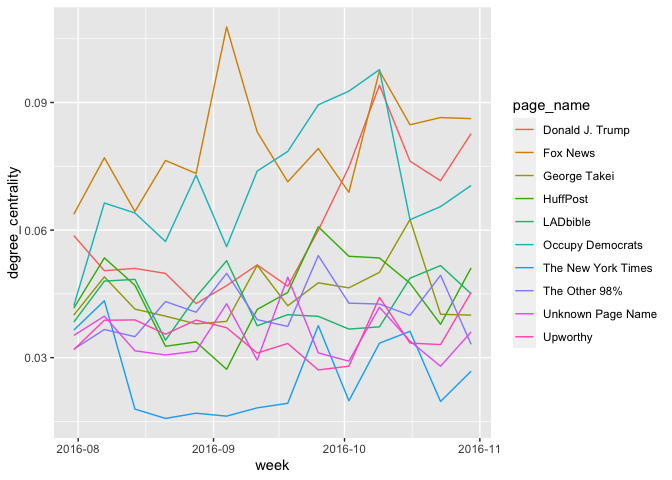
\includegraphics{graph_centrality_files/figure-latex/unnamed-chunk-2-1.pdf}
\#\# Degree Centrality 簡而言之就是總觸及率

\begin{Shaded}
\begin{Highlighting}[]
\NormalTok{centrality }\OtherTok{=} \StringTok{\textquotesingle{}degree\_centrality\textquotesingle{}}
\NormalTok{top.}\FloatTok{10.}\NormalTok{deg }\OtherTok{=} \FunctionTok{get\_top\_10}\NormalTok{(centrality)}
\FunctionTok{plot\_top\_10}\NormalTok{(top.}\FloatTok{10.}\NormalTok{deg, centrality)}
\end{Highlighting}
\end{Shaded}

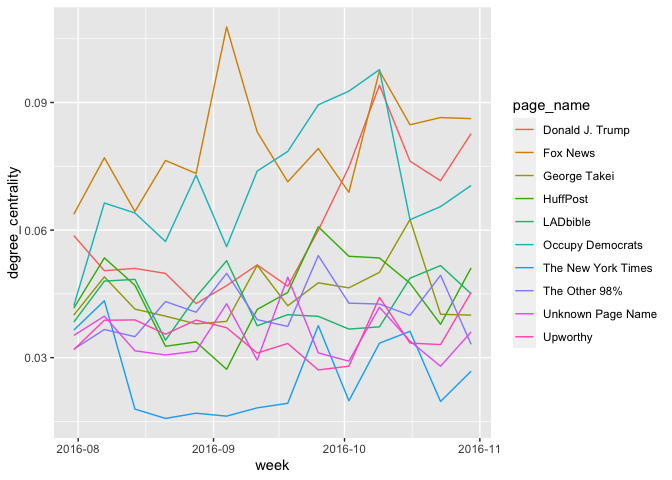
\includegraphics{graph_centrality_files/figure-latex/unnamed-chunk-3-1.pdf}

\hypertarget{eigenvalue-centrality}{%
\subsection{Eigenvalue Centrality}\label{eigenvalue-centrality}}

與結點互動的對象中心性越高,自己的中心性就會越高

\[
C_E^{user} =  \frac{1}{\lambda} \sum_{p \in page} C_E^{page}(p) a_{ip} \\
C_E^{page} =  \frac{1}{\lambda} \sum_{u \in user} C_E^{user}(u) a_{iu}
\]

\begin{Shaded}
\begin{Highlighting}[]
\NormalTok{centrality }\OtherTok{=} \StringTok{\textquotesingle{}eigenvector\_centrality\textquotesingle{}}
\NormalTok{top.}\FloatTok{10.}\NormalTok{eig }\OtherTok{=} \FunctionTok{get\_top\_10}\NormalTok{(centrality)}
\FunctionTok{plot\_top\_10}\NormalTok{(top.}\FloatTok{10.}\NormalTok{eig, centrality)}
\end{Highlighting}
\end{Shaded}

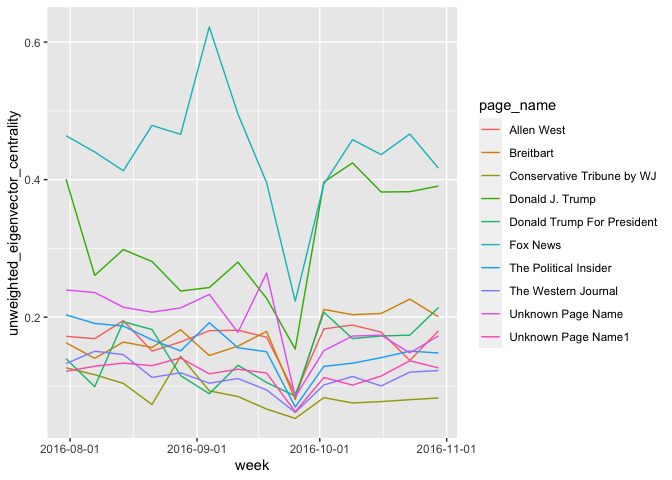
\includegraphics{graph_centrality_files/figure-latex/unnamed-chunk-4-1.pdf}

\begin{Shaded}
\begin{Highlighting}[]
\NormalTok{centrality }\OtherTok{=} \StringTok{\textquotesingle{}unweighted\_eigenvector\_centrality\textquotesingle{}}
\NormalTok{top.}\FloatTok{10.}\NormalTok{unw.eig }\OtherTok{=} \FunctionTok{get\_top\_10}\NormalTok{(centrality)}
\FunctionTok{plot\_top\_10}\NormalTok{(top.}\FloatTok{10.}\NormalTok{unw.eig, centrality)}
\end{Highlighting}
\end{Shaded}

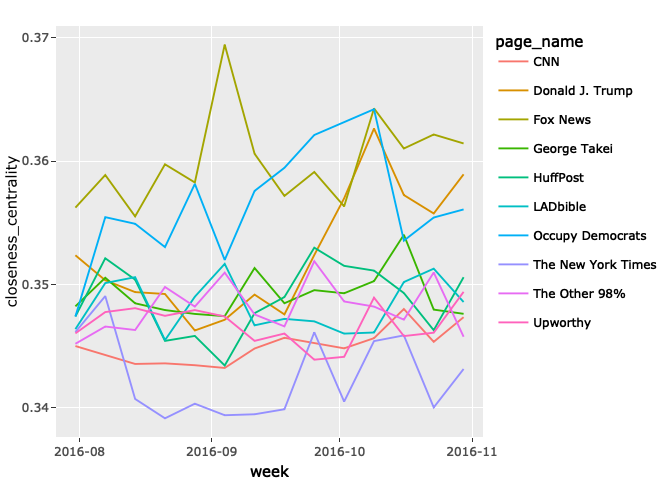
\includegraphics{graph_centrality_files/figure-latex/unnamed-chunk-5-1.pdf}

Narmalize 後容易被 outlire
影響(10月上下,有一個用戶特別勤奮對其中一個粉專按讚,則他與那個粉專的中心性都會增加)

\hypertarget{closeness-centrality}{%
\subsection{Closeness Centrality}\label{closeness-centrality}}

到其他節點的平均距離(次數)越高,中心性越小。

\begin{Shaded}
\begin{Highlighting}[]
\NormalTok{centrality }\OtherTok{=} \StringTok{\textquotesingle{}closeness\_centrality\textquotesingle{}}
\NormalTok{top.}\FloatTok{10.}\NormalTok{cls }\OtherTok{=} \FunctionTok{get\_top\_10}\NormalTok{(centrality)}
\FunctionTok{plot\_top\_10}\NormalTok{(top.}\FloatTok{10.}\NormalTok{cls, centrality)}
\end{Highlighting}
\end{Shaded}

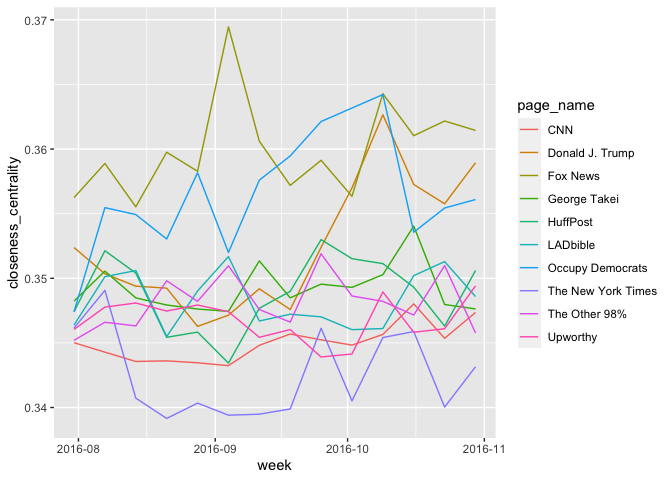
\includegraphics{graph_centrality_files/figure-latex/unnamed-chunk-6-1.pdf}

互動次數在計算過程中不具意義,較不具代表性的衡量

\hypertarget{current-flow-betweenness-centrality}{%
\subsection{Current Flow Betweenness
Centrality}\label{current-flow-betweenness-centrality}}

如果以其中一個粉專/用戶作為消息來源起點(source),另外一個粉專/用戶作為消息終點(sink),則關注的節點對於資訊流量的貢獻有多少?

該節點在每一對節點之間的流量總和,就是Current flow betweenness
centrality。

計算上模擬電流運作 \url{https://tinyurl.com/27dcmgj5}

\hypertarget{what-happned-in-2016-09-25}{%
\subsection{What happned in
2016-09-25?}\label{what-happned-in-2016-09-25}}

\begin{Shaded}
\begin{Highlighting}[]
\CommentTok{\#out.width="100\%"\}}

\NormalTok{top10.unweighted.eig.centrality.week\_other }\OtherTok{=}\NormalTok{ Full\_centrality }\SpecialCharTok{\%\textgreater{}\%} \FunctionTok{filter}\NormalTok{(week }\SpecialCharTok{==} \StringTok{\textquotesingle{}2016{-}09{-}25\textquotesingle{}}\NormalTok{) }\SpecialCharTok{\%\textgreater{}\%} \FunctionTok{arrange}\NormalTok{(}\FunctionTok{desc}\NormalTok{(unweighted\_eigenvector\_centrality)) }\SpecialCharTok{\%\textgreater{}\%} \FunctionTok{select}\NormalTok{(page\_name) }\SpecialCharTok{\%\textgreater{}\%} \FunctionTok{head}\NormalTok{(}\DecValTok{3}\NormalTok{) }\SpecialCharTok{\%\textgreater{}\%}\NormalTok{ pull}


\NormalTok{top10.unweighted.eig.centrality.all }\OtherTok{=}\NormalTok{ Full\_centrality }\SpecialCharTok{\%\textgreater{}\%} \FunctionTok{filter}\NormalTok{(page\_name }\SpecialCharTok{\%in\%} \FunctionTok{c}\NormalTok{(top.}\FloatTok{10.}\NormalTok{unw.eig[}\DecValTok{1}\SpecialCharTok{:}\DecValTok{3}\NormalTok{], top10.unweighted.eig.centrality.week\_other)) }\SpecialCharTok{\%\textgreater{}\%} \FunctionTok{select}\NormalTok{(page\_name,unweighted\_eigenvector\_centrality, week)}


\NormalTok{top10.unweighted.eig.centrality.all }\SpecialCharTok{\%\textgreater{}\%} \FunctionTok{ggplot}\NormalTok{() }\SpecialCharTok{+} 
  \FunctionTok{geom\_line}\NormalTok{(}\FunctionTok{aes}\NormalTok{(}\AttributeTok{y =}\NormalTok{ unweighted\_eigenvector\_centrality, }\AttributeTok{x =}\NormalTok{ week, }\AttributeTok{color=}\NormalTok{page\_name)) }\SpecialCharTok{+}
  \FunctionTok{scale\_x\_date}\NormalTok{(}\AttributeTok{labels =} \FunctionTok{date\_format}\NormalTok{(}\StringTok{"\%Y{-}\%m{-}\%d"}\NormalTok{))}
\end{Highlighting}
\end{Shaded}

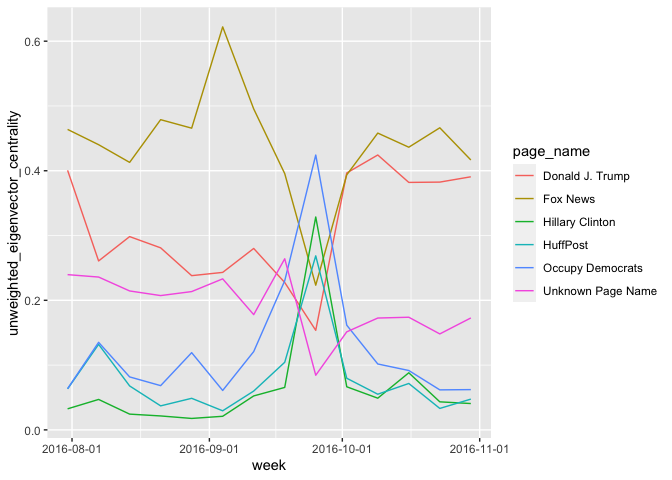
\includegraphics{graph_centrality_files/figure-latex/unnamed-chunk-7-1.pdf}

\begin{Shaded}
\begin{Highlighting}[]
\CommentTok{\#ggplotly(p)}
\end{Highlighting}
\end{Shaded}

\begin{Shaded}
\begin{Highlighting}[]
\CommentTok{\#out.width="100\%"\}}

\NormalTok{top10.eig.centrality.week\_other }\OtherTok{=}\NormalTok{ Full\_centrality }\SpecialCharTok{\%\textgreater{}\%} \FunctionTok{filter}\NormalTok{(week }\SpecialCharTok{==} \StringTok{\textquotesingle{}2016{-}10{-}02\textquotesingle{}}\NormalTok{) }\SpecialCharTok{\%\textgreater{}\%} \FunctionTok{arrange}\NormalTok{(}\FunctionTok{desc}\NormalTok{(eigenvector\_centrality)) }\SpecialCharTok{\%\textgreater{}\%} \FunctionTok{select}\NormalTok{(page\_name) }\SpecialCharTok{\%\textgreater{}\%} \FunctionTok{head}\NormalTok{(}\DecValTok{4}\NormalTok{) }\SpecialCharTok{\%\textgreater{}\%}\NormalTok{ pull}


\NormalTok{top10.eig.centrality.all }\OtherTok{=}\NormalTok{ Full\_centrality }\SpecialCharTok{\%\textgreater{}\%} \FunctionTok{filter}\NormalTok{(page\_name }\SpecialCharTok{\%in\%} \FunctionTok{c}\NormalTok{(top.}\FloatTok{10.}\NormalTok{eig[}\DecValTok{1}\SpecialCharTok{:}\DecValTok{4}\NormalTok{], top10.eig.centrality.week\_other)) }\SpecialCharTok{\%\textgreater{}\%} \FunctionTok{select}\NormalTok{(page\_name,unweighted\_eigenvector\_centrality, week)}


\NormalTok{top10.eig.centrality.all }\SpecialCharTok{\%\textgreater{}\%} \FunctionTok{ggplot}\NormalTok{() }\SpecialCharTok{+} 
  \FunctionTok{geom\_line}\NormalTok{(}\FunctionTok{aes}\NormalTok{(}\AttributeTok{y =}\NormalTok{ unweighted\_eigenvector\_centrality, }\AttributeTok{x =}\NormalTok{ week, }\AttributeTok{color=}\NormalTok{page\_name)) }\SpecialCharTok{+}
  \FunctionTok{scale\_x\_date}\NormalTok{(}\AttributeTok{labels =} \FunctionTok{date\_format}\NormalTok{(}\StringTok{"\%Y{-}\%m{-}\%d"}\NormalTok{))}
\end{Highlighting}
\end{Shaded}

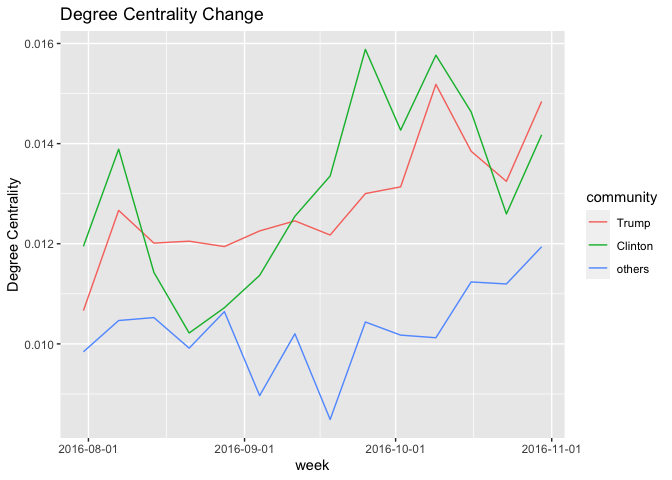
\includegraphics{graph_centrality_files/figure-latex/unnamed-chunk-8-1.pdf}

\begin{Shaded}
\begin{Highlighting}[]
\CommentTok{\#ggplotly(p)}
\end{Highlighting}
\end{Shaded}

\hypertarget{ux793eux7fa4ux5075ux6e2c-community-detection}{%
\section{社群偵測 Community
Detection}\label{ux793eux7fa4ux5075ux6e2c-community-detection}}

將用戶粉專互動的社會網路投影到只有粉專的社會網路上,並以此進行community
detection(透過 Louvain
algorithm),可以大致的偵測出支持川普陣營的粉專,以及希拉蕊陣營的粉專。

以下將各個陣營的粉專的各種中心性取平均,畫出隨時間的變化圖

\begin{Shaded}
\begin{Highlighting}[]
\FunctionTok{library}\NormalTok{(readr)}
\NormalTok{avg\_centrality\_panel }\OtherTok{\textless{}{-}} \FunctionTok{read\_csv}\NormalTok{(}\StringTok{"avg\_centrality\_panel.csv"}\NormalTok{, }
    \AttributeTok{col\_types =} \FunctionTok{cols}\NormalTok{(}\AttributeTok{week =} \FunctionTok{col\_date}\NormalTok{(}\AttributeTok{format =} \StringTok{"\%Y{-}\%m{-}\%d"}\NormalTok{)))}
\NormalTok{avg\_centrality\_panel}\SpecialCharTok{$}\NormalTok{community }\OtherTok{=} \FunctionTok{factor}\NormalTok{(}
\NormalTok{                      avg\_centrality\_panel}\SpecialCharTok{$}\NormalTok{community,}
                      \AttributeTok{levels =} \FunctionTok{c}\NormalTok{(}\StringTok{\textquotesingle{}Trump\textquotesingle{}}\NormalTok{, }\StringTok{\textquotesingle{}Clinton\textquotesingle{}}\NormalTok{,}\StringTok{\textquotesingle{}others\textquotesingle{}}\NormalTok{))}

\NormalTok{plot\_avg\_centrality }\OtherTok{=} \ControlFlowTok{function}\NormalTok{(col\_name, title\_name)\{}
\NormalTok{  avg\_centrality\_panel }\SpecialCharTok{\%\textgreater{}\%} \FunctionTok{ggplot}\NormalTok{() }\SpecialCharTok{+}
  \FunctionTok{geom\_line}\NormalTok{(}\FunctionTok{aes}\NormalTok{(}\AttributeTok{x =}\NormalTok{ week, }\AttributeTok{y =}\NormalTok{ .data[[col\_name]], }\AttributeTok{color =}\NormalTok{ community)) }\SpecialCharTok{+}
  \FunctionTok{scale\_x\_date}\NormalTok{(}\AttributeTok{labels =} \FunctionTok{date\_format}\NormalTok{(}\StringTok{"\%Y{-}\%m{-}\%d"}\NormalTok{)) }\SpecialCharTok{+} 
  \FunctionTok{ggtitle}\NormalTok{(}\FunctionTok{paste}\NormalTok{(title\_name, }\StringTok{"Change"}\NormalTok{)) }\SpecialCharTok{+}
  \FunctionTok{ylab}\NormalTok{(title\_name)}
\NormalTok{\}}

\FunctionTok{plot\_avg\_centrality}\NormalTok{(}\StringTok{\textquotesingle{}degree\_centrality\textquotesingle{}}\NormalTok{, }
                    \StringTok{\textquotesingle{}Degree Centrality\textquotesingle{}}\NormalTok{)}
\end{Highlighting}
\end{Shaded}

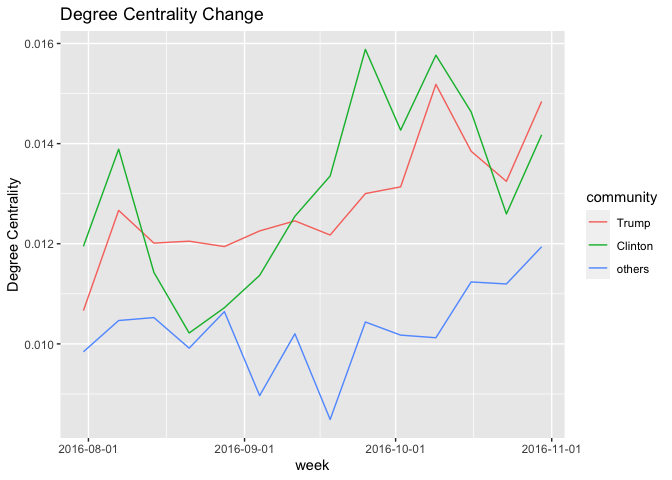
\includegraphics{graph_centrality_files/figure-latex/unnamed-chunk-9-1.pdf}

\begin{Shaded}
\begin{Highlighting}[]
\FunctionTok{plot\_avg\_centrality}\NormalTok{(}\StringTok{\textquotesingle{}eigenvector\_centrality\textquotesingle{}}\NormalTok{, }
                    \StringTok{\textquotesingle{}Eigenvector Centrality\textquotesingle{}}\NormalTok{)}
\end{Highlighting}
\end{Shaded}

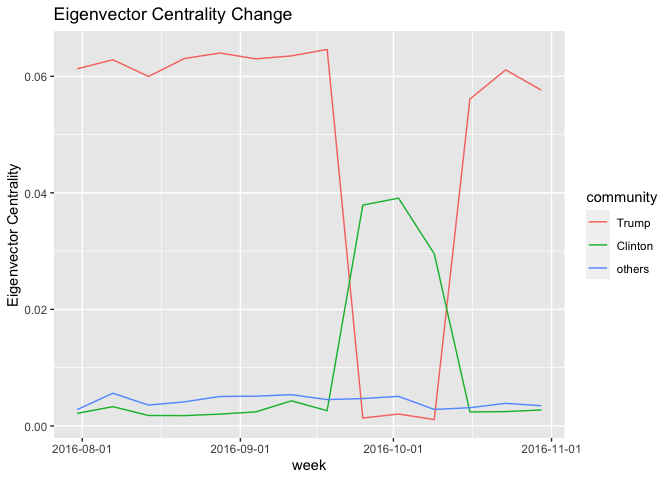
\includegraphics{graph_centrality_files/figure-latex/unnamed-chunk-9-2.pdf}

\begin{Shaded}
\begin{Highlighting}[]
\FunctionTok{plot\_avg\_centrality}\NormalTok{(}\StringTok{\textquotesingle{}unweighted\_eigenvector\_centrality\textquotesingle{}}\NormalTok{, }
                    \StringTok{\textquotesingle{}Unweighted Eigenvector Centrality\textquotesingle{}}\NormalTok{)}
\end{Highlighting}
\end{Shaded}

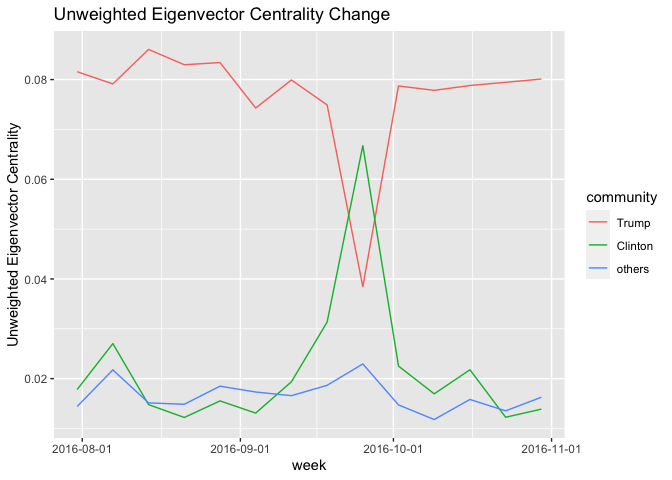
\includegraphics{graph_centrality_files/figure-latex/unnamed-chunk-9-3.pdf}

\begin{Shaded}
\begin{Highlighting}[]
\FunctionTok{plot\_avg\_centrality}\NormalTok{(}\StringTok{\textquotesingle{}closeness\_centrality\textquotesingle{}}\NormalTok{, }
                    \StringTok{\textquotesingle{}Closeness Centrality\textquotesingle{}}\NormalTok{)}
\end{Highlighting}
\end{Shaded}

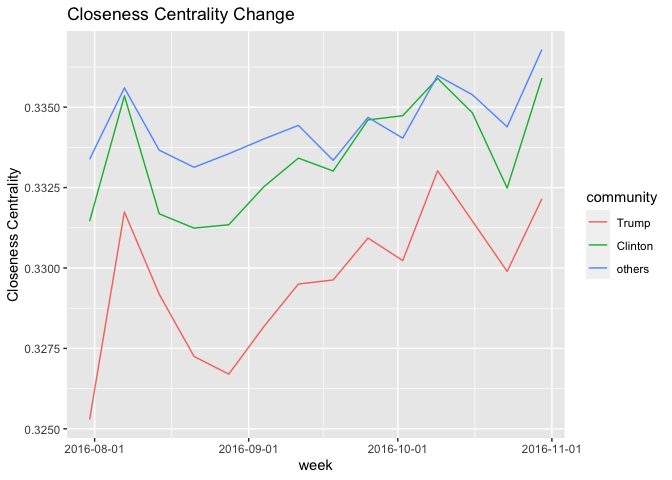
\includegraphics{graph_centrality_files/figure-latex/unnamed-chunk-9-4.pdf}

\hypertarget{ux56deux6b78}{%
\section{回歸}\label{ux56deux6b78}}

回歸結果

input(`Result/reg\_result/deg\_c.tex')

\end{document}
